%\subsection{Tapered waveguide due to interface width} 
%tapered_width
The taper width of the waveguide affects the acceptable scale of light power. It is given in Fig. \ref {fig:Tapered_core_spot_curve}	 that the beam spot diameter at the working distance is about $1.5\mu$m, while the regular waveguide has smaller dimensions (w=$1\mu$m and h=$0.5\mu$m). That means the original waveguide dimension is not adaptable for more incident power. In this section the tapered waveguide is placed at the working distance of $4\mu$m from TLF and the taper width starting with $1.2\mu$m to $3\mu$m with step $0.2\mu$m, taper length is a constant of $5.5\mu$m. \\

\begin{figure}[!ht]
\centering
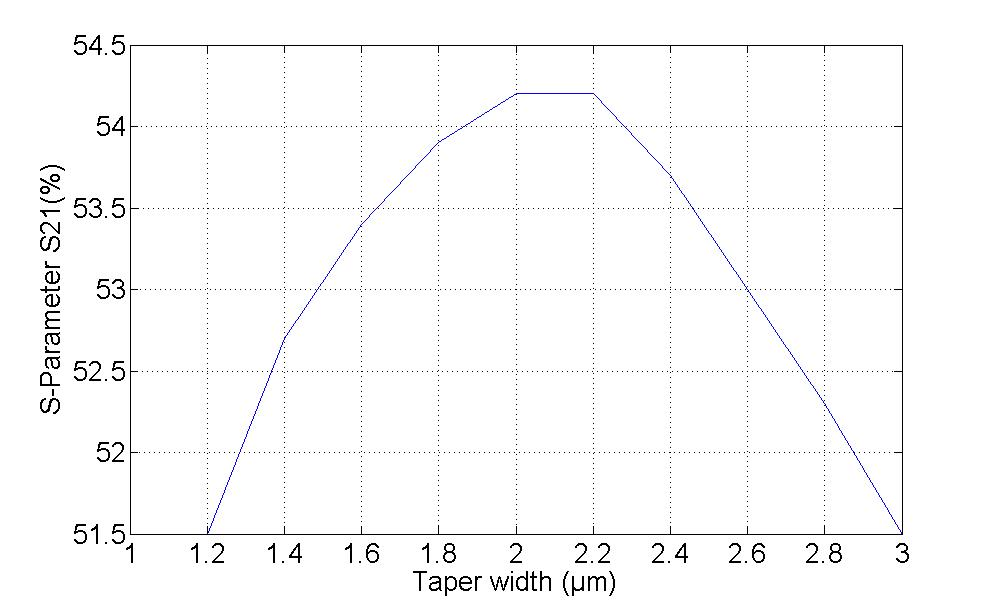
\includegraphics[width=0.7\textwidth]{bilder/tapered_waveguide_wxx}
\caption{Coupling efficiency between TLF and tapered waveguide with constant taper length $= 5.5\mu$m due to the variations of the interface width, working frequency $282$THz.}
\label{fig:tapered_waveguide_wxx}
\end{figure}
Fig. \ref{fig:tapered_waveguide_wxx} exhibits the coupling behavior of the tapered waveguide along the variation of the interface width. From the figure it can be told that the coupling efficiency of this arrangement rises firstly from $51.5\%$ for $d_{1}=1.2\mu$m and achieves the peak value of about $54.2\%$ for the taper width $d_{1}=2\mu$m and $2.2\mu$m. Then the efficiency falls as the taper width increasing. This tendency can be explained that a wider interface can confine more incident rays into the propagation tunnel, but if the interface expands continually, other aspects, such as the divergence angle, may cause the decline of the coupling ability over the effect of the interface width.  That means, an efficient taper structure depends not only on taper width.  In next subsection we will discuss another property of the taper structure.\\ 

